\documentclass[14pt]{extbook}
\usepackage{multicol, enumerate, enumitem, hyperref, color, soul, setspace, parskip, fancyhdr} %General Packages
\usepackage{amssymb, amsthm, amsmath, bbm, latexsym, units, mathtools} %Math Packages
\everymath{\displaystyle} %All math in Display Style
% Packages with additional options
\usepackage[headsep=0.5cm,headheight=12pt, left=1 in,right= 1 in,top= 1 in,bottom= 1 in]{geometry}
\usepackage[usenames,dvipsnames]{xcolor}
\usepackage{dashrule}  % Package to use the command below to create lines between items
\newcommand{\litem}[1]{\item#1\hspace*{-1cm}\rule{\textwidth}{0.4pt}}
\pagestyle{fancy}
\lhead{Makeup Progress Quiz 3}
\chead{}
\rhead{Version C}
\lfoot{4315-3397}
\cfoot{}
\rfoot{Fall 2020}
\begin{document}

\begin{enumerate}
\litem{
Find the equation of the line described below. Write the linear equation as $ y=mx+b $ and choose the intervals that contain $m$ and $b$.\[ \text{Parallel to } 8 x + 7 y = 4 \text{ and passing through the point } (-10, -10). \]\begin{enumerate}[label=\Alph*.]
\item \( m \in [-2.13, -0.99] \hspace*{3mm} b \in [21.37, 22.44] \)
\item \( m \in [-1.04, 0.25] \hspace*{3mm} b \in [-21.6, -19.86] \)
\item \( m \in [0.9, 1.41] \hspace*{3mm} b \in [0.01, 1.59] \)
\item \( m \in [-2.13, -0.99] \hspace*{3mm} b \in [-1.13, 1.27] \)
\item \( m \in [-2.13, -0.99] \hspace*{3mm} b \in [-21.6, -19.86] \)

\end{enumerate} }
\litem{
Solve the equation below. Then, choose the interval that contains the solution.\[ -9(-6x -5) = -8(14x + 13) \]\begin{enumerate}[label=\Alph*.]
\item \( x \in [-1.28, -0.99] \)
\item \( x \in [-0.9, -0.79] \)
\item \( x \in [-0.52, -0.32] \)
\item \( x \in [0.28, 0.47] \)
\item \( \text{There are no real solutions.} \)

\end{enumerate} }
\litem{
Solve the equation below. Then, choose the interval that contains the solution.\[ -4(11x -19) = -2(12x -10) \]\begin{enumerate}[label=\Alph*.]
\item \( x \in [-6.8, -1.8] \)
\item \( x \in [3.8, 6.8] \)
\item \( x \in [-2.59, 2.41] \)
\item \( x \in [1.8, 3.8] \)
\item \( \text{There are no real solutions.} \)

\end{enumerate} }
\litem{
Solve the linear equation below. Then, choose the interval that contains the solution.\[ \frac{7x + 3}{5} - \frac{-5x -6}{6} = \frac{9x -3}{4} \]\begin{enumerate}[label=\Alph*.]
\item \( x \in [720, 721] \)
\item \( x \in [21, 23] \)
\item \( x \in [140, 142] \)
\item \( x \in [-4.78, 1.22] \)
\item \( \text{There are no real solutions.} \)

\end{enumerate} }
\litem{
First, find the equation of the line containing the two points below. Then, write the equation as $ y=mx+b $ and choose the intervals that contain $m$ and $b$.\[ (-11, -4) \text{ and } (-6, -10) \]\begin{enumerate}[label=\Alph*.]
\item \( m \in [1.2, 2.2] \hspace*{3mm} b \in [-3.1, -2.1] \)
\item \( m \in [-4.2, -0.2] \hspace*{3mm} b \in [-7.2, -3.8] \)
\item \( m \in [-4.2, -0.2] \hspace*{3mm} b \in [6.3, 10.3] \)
\item \( m \in [-4.2, -0.2] \hspace*{3mm} b \in [16.5, 21.3] \)
\item \( m \in [-4.2, -0.2] \hspace*{3mm} b \in [-18.1, -16.1] \)

\end{enumerate} }
\litem{
Write the equation of the line in the graph below in Standard form $Ax+By=C$. Then, choose the intervals that contain $A, B, \text{ and } C$.
\begin{center}
    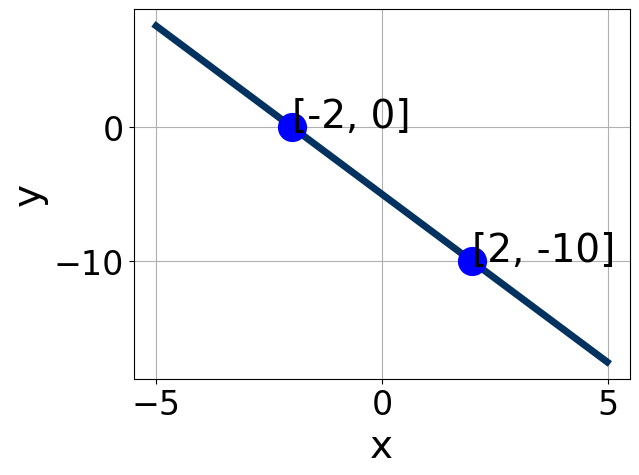
\includegraphics[width=0.5\textwidth]{../Figures/linearGraphToStandardCopyC.png}
\end{center}
\begin{enumerate}[label=\Alph*.]
\item \( A \in [1.2, 4.7], \hspace{3mm} B \in [-1.7, -0.31], \text{ and } \hspace{3mm} C \in [3, 6] \)
\item \( A \in [-8, -4.2], \hspace{3mm} B \in [-2.07, -1.25], \text{ and } \hspace{3mm} C \in [7, 13] \)
\item \( A \in [1.2, 4.7], \hspace{3mm} B \in [0.3, 1.2], \text{ and } \hspace{3mm} C \in [-8, 0] \)
\item \( A \in [2.9, 5.4], \hspace{3mm} B \in [1.53, 2.46], \text{ and } \hspace{3mm} C \in [-11, -9] \)
\item \( A \in [2.9, 5.4], \hspace{3mm} B \in [-2.07, -1.25], \text{ and } \hspace{3mm} C \in [7, 13] \)

\end{enumerate} }
\litem{
Write the equation of the line in the graph below in Standard form $Ax+By=C$. Then, choose the intervals that contain $A, B, \text{ and } C$.
\begin{center}
    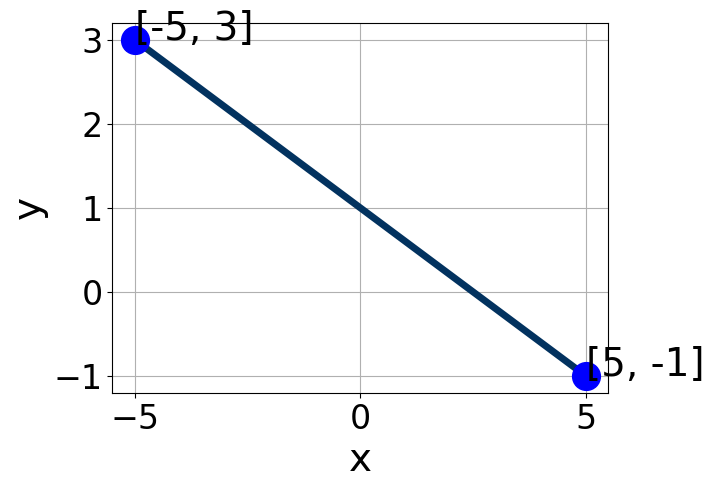
\includegraphics[width=0.5\textwidth]{../Figures/linearGraphToStandardC.png}
\end{center}
\begin{enumerate}[label=\Alph*.]
\item \( A \in [-3.2, -1.62], \hspace{3mm} B \in [-6.4, -3], \text{ and } \hspace{3mm} C \in [-5.2, -3.1] \)
\item \( A \in [1.66, 2.77], \hspace{3mm} B \in [-6.4, -3], \text{ and } \hspace{3mm} C \in [-5.2, -3.1] \)
\item \( A \in [1.66, 2.77], \hspace{3mm} B \in [3.1, 6.8], \text{ and } \hspace{3mm} C \in [3.7, 8.7] \)
\item \( A \in [-1.47, 0.43], \hspace{3mm} B \in [0.9, 1.2], \text{ and } \hspace{3mm} C \in [-0.1, 1.4] \)
\item \( A \in [-1.47, 0.43], \hspace{3mm} B \in [-1.1, -0.9], \text{ and } \hspace{3mm} C \in [-1.3, 0.2] \)

\end{enumerate} }
\litem{
First, find the equation of the line containing the two points below. Then, write the equation as $ y=mx+b $ and choose the intervals that contain $m$ and $b$.\[ (4, 10) \text{ and } (-9, 2) \]\begin{enumerate}[label=\Alph*.]
\item \( m \in [0.43, 1.79] \hspace*{3mm} b \in [3, 7] \)
\item \( m \in [0.43, 1.79] \hspace*{3mm} b \in [6.54, 9.54] \)
\item \( m \in [0.43, 1.79] \hspace*{3mm} b \in [10, 20] \)
\item \( m \in [0.43, 1.79] \hspace*{3mm} b \in [-11.54, -6.54] \)
\item \( m \in [-2.34, 0.24] \hspace*{3mm} b \in [-3.54, 3.46] \)

\end{enumerate} }
\litem{
Find the equation of the line described below. Write the linear equation as $ y=mx+b $ and choose the intervals that contain $m$ and $b$.\[ \text{Parallel to } 3 x + 8 y = 8 \text{ and passing through the point } (3, -2). \]\begin{enumerate}[label=\Alph*.]
\item \( m \in [-3.19, -2.38] \hspace*{3mm} b \in [-2.1, 0.5] \)
\item \( m \in [-0.22, 0.95] \hspace*{3mm} b \in [-4.4, -1.1] \)
\item \( m \in [-1.02, -0.27] \hspace*{3mm} b \in [-2.1, 0.5] \)
\item \( m \in [-1.02, -0.27] \hspace*{3mm} b \in [-0.2, 1.5] \)
\item \( m \in [-1.02, -0.27] \hspace*{3mm} b \in [-6.1, -4.8] \)

\end{enumerate} }
\litem{
Solve the linear equation below. Then, choose the interval that contains the solution.\[ \frac{-8x -9}{5} - \frac{-4x -3}{8} = \frac{-7x -9}{7} \]\begin{enumerate}[label=\Alph*.]
\item \( x \in [27, 32] \)
\item \( x \in [-9.89, -7.89] \)
\item \( x \in [-4.39, -0.39] \)
\item \( x \in [-0.95, 1.05] \)
\item \( \text{There are no real solutions.} \)

\end{enumerate} }
\end{enumerate}

\end{document}